% 
% Annual Cognitive Science Conference
% Sample LaTeX Paper -- Proceedings Format
% 

% Original : Ashwin Ram (ashwin@cc.gatech.edu)       04/01/1994
% Modified : Johanna Moore (jmoore@cs.pitt.edu)      03/17/1995
% Modified : David Noelle (noelle@ucsd.edu)          03/15/1996
% Modified : Pat Langley (langley@cs.stanford.edu)   01/26/1997
% Latex2e corrections by Ramin Charles Nakisa        01/28/1997 
% Modified : Tina Eliassi-Rad (eliassi@cs.wisc.edu)  01/31/1998
% Modified : Trisha Yannuzzi (trisha@ircs.upenn.edu) 12/28/1999 (in process)
% Modified : Mary Ellen Foster (M.E.Foster@ed.ac.uk) 12/11/2000
% Modified : Ken Forbus                              01/23/2004
% Modified : Eli M. Silk (esilk@pitt.edu)            05/24/2005
% Modified : Niels Taatgen (taatgen@cmu.edu)         10/24/2006
% Modified : David Noelle (dnoelle@ucmerced.edu)     11/19/2014

%% Change "letterpaper" in the following line to "a4paper" if you must.

\documentclass[10pt,letterpaper]{article}

\usepackage{cogsci}
\usepackage{pslatex}
\usepackage{apacite}
\usepackage{graphicx}
\usepackage{url}

\title{Genericity and Reference Failure}
 
\author{{\large \bf Phil Crone} \\
	\texttt{pcrone@stanford.edu}\\
  Department of Linguistics \\
  Stanford University
  \And {\large \bf Michael C. Frank} \\
  \texttt{mcfrank@stanford.edu}\\
  Department of Psychology \\
  Stanford University}

\begin{document}

\maketitle

\begin{abstract}
Generic sentences (e.g., ``birds lay eggs'') express generalizations about kinds, rather than facts about specific individuals or sets of individuals (e.g., ``all birds lay eggs''). Although generics are pervasive in natural language, there is no unique linguistic marker of genericity, making the identification of generics a challenge. We investigate the morphosyntactic cues that listeners use to identify whether a sentence should receive a generic interpretation or not. We find that two factors -- the definiteness of a sentence's subject NP and the tense of the sentence -- are extremely important in guiding intuitions about whether a sentence should receive a generic interpretation. We argue that the importance of these factors can be explained by taking generic interpretations to arise due to a failure to ground expressions as referring to specific entities or events. 

\textbf{Keywords:} Psycholinguistics; pragmatics; generics.
\end{abstract}


\section{Introduction}
 
Generic sentences express generalizations about kinds rather than individuals and are an important route for the transmission of knowledge \cite{gelman2003}. A key difference between generic and non-generic statements is that generics allow for exceptions: ``birds fly'' expresses a generalization about the kind \textit{bird} and is true despite the fact that some birds do not fly, while ``all birds fly'' is false, because, e.g., emus do not fly \cite{Prasada:2000}. 

Generics are not consistently marked by any particular lexical, morphological, or syntactic convention, so how do we know that a sentence is generic? Prior work suggest at least three types of cues that guide the interpretation of sentences as generic or non-generic: morphosyntactic features, pragmatic cues, and world knowledge. In English, the subject noun phase (NP) of a generic sentence is often a bare plural (``birds fly''), but it can also be an indefinite singular (``a bird has feathers'') or definite singular (``the bird is a warm-blooded animal''). In contrast, definite plural subject NPs (``the birds have beaks'') are generally thought to force non-generic interpretations. Tense and aspect also cue whether a sentence is interpreted generically; simple present tense (``birds fly'') is more associated with generic meanings than, e.g., present progressive (``birds are flying overhead'') or past (``birds flew by my window'') \cite{Carlson:1977,Krifka:1995,Lyons:1977}. 

Pragmatics and world knowledge also influence a sentence's interpretation as generic or non-generic. For example, if a unique bird is present in the context of an utterance of a sentence with the subject NP ``the bird,'' this NP is likely to be interpreted as referring to the bird in context, giving rise to a non-generic interpretation. Conversely, if no such bird exists in the context, a generic interpretation may be preferred. Finally, world knowledge about properties shared by members of a kind influences the interpretation of potentially generic sentences. The sentence ``a bird does not fly'' is interpreted as being about some particular bird (e.g., a penguin), given world knowledge that, in general, birds fly. 

Previous experimental work has confirmed the influence of morphosyntax, pragmatic context, and world knowledge on the interpretation of sentences as generic. Adults and children can use the definiteness of subject NPs, as well as tense and aspect, to identify generics, and prefer generic interpretations when the subject NP has no available referent in context \cite{Gelman:2003,Cimpian:2011}. By age 3, children are less likely to assign a generic interpretation to a sentence when its subject NP has a possible referent in the preceding linguistic context and can also use knowledge about the generalizability of properties to kinds in identifying generics \cite{Cimpian:2008}.

The present studies build on this prior work, but differs from previous studies in several ways. First, we focus on the quantitative relationship between factors in adults' recognition of generics. Most previous work on the identification of generics has focused on children's abilities, perhaps stemming in part from an assumption that children face challenges in identifying generics that are less relevant for adults. However, research on the probabilistic nature of language comprehension suggests that adults face a similar problem \cite{Levy:2008,Frank:2012}. In the case of identifying generics, we can take adults to reason about the likelihood that an utterance is generic given morphosyntactic features of the sentence, features of the context, and the their own world knowledge. Second, we collect naturalistic examples of generic and non-generic sentences generated by study participants, allowing us to consider a realistic representation of genericity in natural language. In addition, we synthesize the results of the present and previous studies by arguing that generic interpretations of sentences are driven by a failure to identify a referent for entities or events described by the sentence. 

We first introduce an experimental paradigm that allows us to gather a large number of naturalistic examples of generic and non-generic sentences from study participants. We then collect judgments from a second, independent set of participants, as to whether these sentences should receive generic or non-generic interpretations (Experiment 1). We next use several machine learning techniques to identify which factors are most useful in classifying sentences as generic or not. We find that just two factors, definiteness of the subject NP and tense, prove extremely successful in classifying sentences. Finally, we validate the importance of tense for generic interpretation with human subjects (Experiment 2). Taken together, the results of these experiments show that judgments of whether a sentence is generic or non-generic can largely be explained by considering whether the sentence can be referentially grounded.

\section{Experiment 1}

As discussed above, it has been argued that the number and definiteness of a sentence's subject NP influence its interpretation as generic or non-generic \cite{Carlson:1977,Krifka:1995,Lyons:1977}. Previous work investigating these cues to genericity have fixed the number of the subject NP as either singular \cite{Cimpian:2011} or plural \cite{Gelman:2003} and only manipulated definiteness. In Experiment 1, we considered the effects of number, definiteness, and their interaction on the interpretation of generics. Participants performed a sentence completion task in which the subject NP was provided. They then indicated whether the sentences they produced were about specific individuals or kinds.

\begin{table*}
\begin{center} 
\caption{Example Productions from Experiment 1.} 
\label{tab:ex} 
\vskip 0.12in
\begin{tabular}{cccc} 
\hline
Definiteness    &  Number & Genericity & Examples \\
\hline
Indefinite        &   Singular & Generic & ``An elephant is large.'', ``A car is a form of transportation.''\\
Indefinite  &   Singular & Non-generic & ``A dolphin swam alongside the boat.'', ``A guitar kept me up all night.''\\
Indefinite           &   Plural & Generic & ``Foxes chase rabbits.'', ``Computers have made communication easier.''\\
Indefinite         &   Plural  & Non-generic & ``Owls were perched in the barn.'', ``Marbles rolled all over the floor.''\\
Definite        &   Singular & Generic & ``The peacock is a noisy bird.'', ``The chair has four legs.''  \\
Definite  &   Singular & Non-generic & ``The pigeon landed on the car.'', ``The trumpet was out of tune.''\\
Definite           &   Plural & Generic & ``The kangaroos jump a lot.'', ``The guitars are stringed instruments.'' \\
Definite         &   Plural & Non-generic & ``The pandas ate bamboo.'', ``The fences were strong.''\\
\hline
\end{tabular} 
\end{center} 
\end{table*}

\subsection{Method}

\subsubsection{Participants} 

We recruited two sets of participants to participate through Amazon's Mechanical Turk website, with each set of participants performing a different task. We restricted participants to individuals within the United States and paid all participants 50 cents. The sets consisted of 100 and 94 participants, respectively. The first task took approximately 14 minutes to complete, while the second task took approximately 6 minutes. We excluded from the analysis 4 participants from the first set and 6 participants from the second set who indicated that their native language was not English.

\subsubsection{Stimuli}  

For the first set of participants, forty-eight nouns, split evenly between animates and inanimates, were chosen to use as the bases for subject NPs. For each participant, each noun was randomly assigned morphosyntactic features using a \(2 \times 2\) factorial design crossing number (singular, plural) with definiteness (definite, indefinite). Full NPs were created from the base noun and number and definiteness features. For example, if the noun ``panda'' were assigned values \textit{plural} and \textit{definite}, the full NP would be ``the pandas.'' Participants then saw a sequence of each of these NPs followed by a text box. They were instructed to ``write a sentence starting with the phrase below.''

All sentences generated in part 1 by self-reported native English speakers were then split into random sets of approximately 50 sentences each. In part 2, each of these sets of sentences was presented in random order to one participant from the second set of participants. For a sentence whose subject NP was \textit{noun}, participants indicated whether they thought the sentence was about ``\textit{nouns},'' ``a specific \textit{noun}'' (for sentences with singular subject NPs), or ``a specific group of \textit{nouns}'' (for sentences with plural subject NPs).\footnote{Participants included in part 1 also judged whether the sentences that they produced were generic or non-generic in a similar manner. Their responses are not reported here, but were largely similar to the results obtained in part 2.}

\subsubsection{Procedure} 

In part 1, we first presented participants with four example NPs. After providing a sentence completion for each example item, participants were shown an example sentence completion that they could have written for the given NP. These sentences were constructed to favor non-generic interpretations for all NP types. Next, all forty-eight subject NPs were presented in pseudorandom order, counterbalanced so that no two consecutive NPs matched in both number and definiteness. We required participants to provide a sentence completion at least six characters in length for each item. After providing sentence completions for all NPs, participants reported their native language.

In part 2, participants were instructed that they would be viewing a sequence of approximately 50 sentences that had been produced by other Mechanical Turk workers. Participants began by judging 4 example sentences constructed us for which the participants received feedback. The remaining sentences were presented in random order. After completing part 2, participants reported their native language. We measured reaction times for each item, measured from the time the item was presented until the time a response was submitted.  In analyzing results from part 2, we excluded responses whose reaction times were greater than 2 standard deviations from the mean.

% \subsubsection{Data Analysis} 

\subsection{Results and Discussion}

We found that both definiteness and number affected judgments of sentences as generic or non-generic (Figure \ref{fig:e2}). Sentences with indefinite subject NPs---especially ``bare plural'' subjects---were more likely to be rated generic (see Table \ref{tab:ex} for examples).

\begin{figure}[t]
\centering
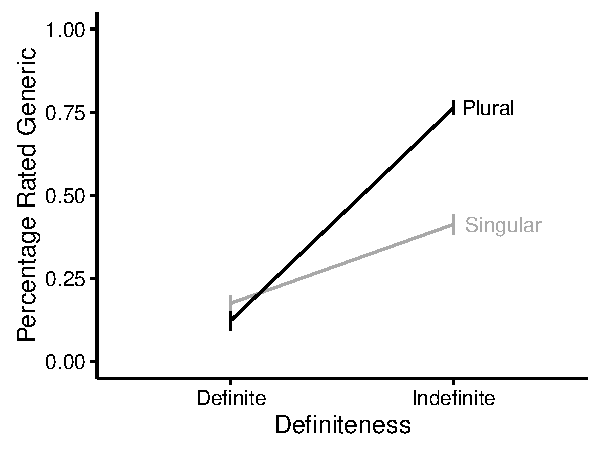
\includegraphics[width=.8\linewidth]{figures/e2-2016.pdf}
\caption{\label{fig:e2} Percentage of sentences rated generic in Experiment 1 by definiteness and number. Error bars show 95\% confidence intervals.} 
\end{figure}

We fit a logistic mixed-effects model to predict a sentence's classification as generic or not from the interaction between definiteness, number, and animacy of the subject NP.\footnote{All data and code can be viewed at \url{https://github.com/langcog/generic_ref}.} The model identified significant main effects of definiteness such that sentences with indefinite subject NPs were more likely to be rated generic (\(\beta = 3.29, z = 14.41, p < 0.001\)) and animacy such that sentences with inanimate subjects were less likely to be rated generic (\(\beta = -1.29, z = -3.33, p < 0.001\)). There were also significant interactions between animacy and definiteness such that sentences with inanimate, indefinite subjects were more likely to be rated generic (\(\beta = 0.86, z = 2.52, p < 0.05\)) and between definiteness and number such that sentences with indefinite, singular subjects were less likely to be rated generic (\(\beta = -1.84, z = -7.59, p < 0.001\)).

The results are consistent with previous findings that indefinite singulars and bare plurals facilitate generic interpretations compared to definite singulars and definite plurals, respectively \cite{Cimpian:2011, Gelman:2003}. The interaction between definiteness and plurality reveals a superadditive effect by which indefinite, bare plurals were rated more generic than would be predicted by the main effects of indefinitenes and plurality. This is unsurprising, as bare plurals are often taken to be the canonical subject type for English generics. The effect of animacy is also consistent with previous findings that both children and adults produce more generic statements when describing animals than when describing artifacts \cite{Brandone:2009}.

Comparing the effect sizes of all significant predictors, we find that definiteness had the greatest influence on participants' responses. Why would this be so? This finding is straightforwardly interpretable in terms of the general hypothesis that generic interpretation arises from reference failure. Since the definite determiner \textit{the}, unlike indefinite determiners, is generally taken to presuppose the existence of a unique, salient entity, it follows that definite subject NPs are more likely to refer to some particular entity. Therefore, sentences with such subjects are less likely to have an intended generic interpretation.

One unexpected finding is that sentences with all subject NP types, including plural definites, were occasionally judged to be generic. This seems to clash with the general view that definite singulars, but not definite plurals, allow for generic interpretations in English. This result forced us consider whether our methodology measured some property other than genericity. However, inspection of definite plurals that were judged generic suggested that these ratings were at least \emph{prima facie} appropriate (Table \ref{tab:ex}). Moreover, recent work has suggested that sentences with definite plural subject NPs in English can receive generic interpretations, at least in certain circumstances \cite{FarkasDeSwart2007}, but that such uses may come with additional social meaning \cite{Acton:2014}. 

\section{Classifying Generics}

In Experiment 1, we directly manipulated the definiteness, number, and animacy features of subject NPs to see what influence these factors would have on the interpretation of sentences as generic or not. However, the sentences produced in Experiment 1 varied in many morphosyntactic, lexical, and semantic respects that we did not directly control. It is plausible that these factors also contributed to judgments in part 2 regarding sentences' classification as generic or not. To probe the influence of these factors on participants' respones, we extracted additional linguistic features from the sentences produced in Experiment 1 and then employed a number of classification techniques to determine which were more important in determining whether a sentence would be judged generic.  

\subsection{Method}

We first used the Stanford part-of-speech (POS) tagger \cite{Toutanova:2003} to obtain POS tags for all sentences judged in Experiment 1. Using these POS tags, we automatically extracted the following features for each sentence: tense, aspect, presence of main verb \textit{be} or \textit{have}, and presence of a modal. We also extract total sentence length minus the length of the subject NP for each sentence.

We next split the sentences produced in Experiment 1 into training and test sets, with the training set consisting of 75\% of all sentences produced. This training set was used to train a variety of classification models, all of which included definiteness, number, and animacy of the subject NP, as well as the factors extracted using the POS tags. Models included generalized linear models, basic decision trees, boosted decision trees, and random forests. Model parameters were optimized using 10-fold cross-validation on the training set. The resulting models were then evaluated against the 25\% held-out test set. All classification techniques achieved test accuracy between 85\% and 87\%. The most straightforwardly interpretable of these methods is the basic decision tree pruned to have three terminal nodes (Figure \ref{fig:tree}). This decision tree, which considers only the definiteness of the subject NP and the tense of the sentence,  achieved a test accuracy of 86.7\%.

\begin{figure}[t]
\centering
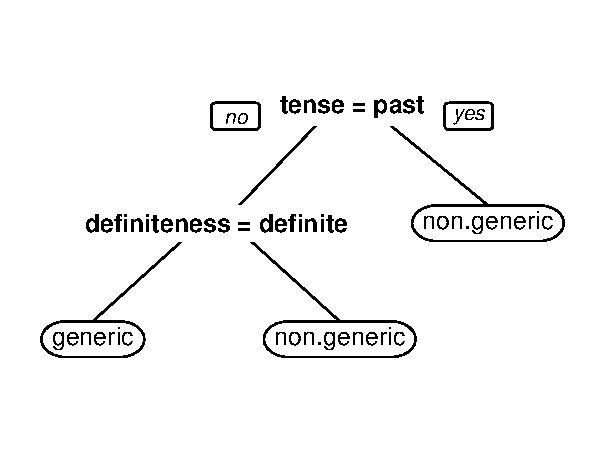
\includegraphics[width=.8\linewidth]{figures/tree.pdf}
\caption{\label{fig:tree} Decision tree with three terminal nodes for classification of sentences as generic or non-generic.} 
\end{figure}

In addition, we had an independent set of participants re-rate the sentences in the held-out test set. The experimental details were the same as those for part 2 of Experiment 1. A total of 41 participants were recruited, all of whom reported that their native language was English. This agreement between these judgments and those collected in Experiment 1 was substantial: the judgments were in agreement 87.8\% of the time, virtually identical to the accuracy of the machine classification techniques we employed, and Cohen's \(\kappa = 0.73\).

\subsection{Results \& Discussion}

The most striking finding in our attempt to classify sentences as generic was that the vast majority of factors considered did not prove useful in this classification task. In the end, we were able to achieve human-level accuracy in the classification task using only the definiteness of a sentence's subject NP and the tense of the sentence. In the discussion of Experiment 1, we already addressed the reason why definiteness might be crucial in guiding generic interpretations. Since the definite article presupposes the existence of a unique, salient entity, a listener can infer that the speaker intended to refer to some particular individual, rather than a kind. 

The importance of tense can be understood in a similar manner. Partee famously observed that the past tense in English has a referential character \cite{Partee:1973}. For example, if I utter ``I didn't turn off the stove,'' this neither means that there is no time in the past at which I turned off the stove (which is false) or that there is any time in the past at which I did not turn off the stove (which is trivially true). Rather, it refers to a particular, relevant interval of time during which I did not turn off the stove. More generally, simple past tense clauses in English refer to particular intervals of time in the past during which particular events occurred. The vast majority (92\%) of non-past sentences produced in Experiment 1 used simple present tense, which is typically used in English to express habits or ongoing states, so long as these hold true at the time of utterance.

We propose that the influence of definiteness and tense on the interpretation of sentences as generic or non-generic can be explained by a single generalization. Listeners attempt to referentially ground the expressions in particular entities or events. Failure to identify referents for these expressions gives rise to generic interpretations.

\section{Experiment 2}

The results of the classification task described above suggest that tense plays a critical role in guiding judgments as to whether a sentence should be interpreted as generic. In order to confirm this finding, we  

\subsection{Method}

\subsubsection{Participants} 

Recruitment details were similar to those of part 2 in Experiment 1. We recruited a total of 50 participants, all of whom were self-reported native English speakers.

\subsubsection{Stimuli}  

We chose a set of 48 sentences that were produced in Experiment 1, one for each base subject noun used in experiment 1. All subject NP types, crossing definiteness, number, and animacy, were equally represented in this set. None of the selected sentences contained main verb \textit{be} or \textit{have}, a modal, or a passive construction. The selected sentences were evenly split between those with simple present and simple past tense verbs. In several cases, sentences produced in Experiment 1 were slightly altered to avoid awkward phrasing or to change the definiteness or number feature of the subject NP to ensure that all pairs of number and definiteness features were equally represented. 

Once all 48 sentences were collected, we created alternate versions of each sentence in which the tense of the main verb was changed from simple present to simple past or vice versa.  

\subsubsection{Procedure} 

The procedure was similar to that of part 2 in Experiment 1. Participants began by judging four example sentences, as in Experiment 1. After this, participants viewed all 48 sentences in random order and indicated whether the sentence was about ``\textit{nouns}'' or ``a specific \textit{noun}/group of \textit{nouns}.'' Half of sentences judged by each participant contained simple present tense verbs, while half contained simple past tense verbs. The order of tenses used in the stimuli was randomized.  

\subsection{Results and Discussion}

\begin{figure}[t]
\centering
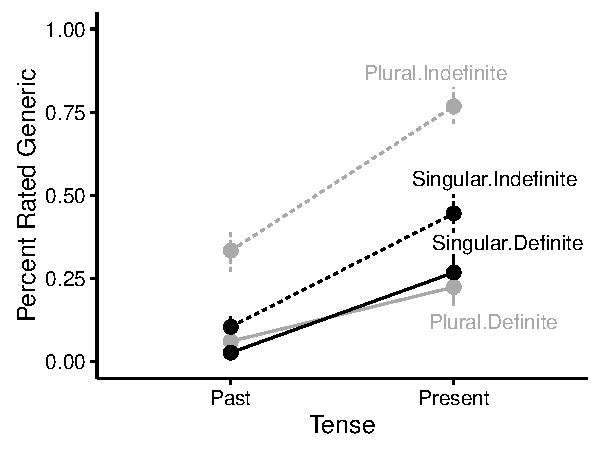
\includegraphics[width=.8\linewidth]{figures/tense.pdf}
\caption{\label{fig:tense} Percentage of sentences rated generic in Experiment 2 by tense, definiteness, and number. Error bars show 95\% confidence intervals.} 
\end{figure}

The effects of definiteness and number of the subject NP were broadly similar to the effects found in Experiment 1. In addition, the tense manipulation appeared to greatly influence judgments, with present tense sentences being more likely to be judged generic across all subject NP types (Figure \ref{fig:tense}).

We fit a logistic mixed-effects model to predict a sentence's classification as generic or non-generic from the interaction of tense, definiteness, number, and animacy. The resulting model revealed only two significant effects; sentences with indefinite subject NPs were more likely to be judged generic (\(\beta = 2.81, z = 3.04, p < 0.01\)), as were present tense sentences (\(\beta = 2.31, z = 3.26, p < 0.01\)). These results provide further confirmation of the findings of the generics classification task. Once again, we find that tense and definiteness are crucial factors that guide interpretation of sentences as either generic or non-generic.

\section{General Discussion}

We set out to explore the question of what gives rise to generic interpretations of sentences. The results here replicate previous findings about cues to genericity: Indefinite subject NPs support generic interpretations more than definite subject NPs \cite{Cimpian:2011, Gelman:2003}, present tense sentences are more likely to be judged generic than past tense sentences \cite{Cimpian:2011}, and sentences with animate subjects tend to be more generic than those with inanimate subjects \cite{Brandone:2009}. However, we found that the most important factors for identifying generic statements were the definiteness of the sentence's subject NP and the tense of the sentence. We have argued that the importance of these two factors can be explained by viewing generic interpretations as the result of listeners' failure to ground expressions as referring to particular entities or events.

This explanation has the potential to explain other factors that have previously been shown to serve as cues to generic meaning. Although we did not find aspect to play a crucial role in classifying sentences as generic or not, previous work has found that both children and adults are more likely to interpret present progressive sentences as non-generic than simple present sentences \cite{Cimpian:2011}. Our failure to identify aspect as a crucial cue to generic meaning is likely due to the fact that only 6.8\% of the sentences produced in Experiment 1 used progressive or perfect aspect. However, our explanation of the nature of generic interpretations is amenable to taking aspect to play a role in determining generic meaning. Events described with the present progressive in English refer to events that are occurring at the speech time. Therefore, a listener can infer from a sentence using the present progressive that a speaker intended to refer to a particular event.

Our proposal also straightforwardly explains previous findings that the contextual availability of a referent for the subject NP of a sentence makes it more likely that the sentence will be judged non-generic \cite{Gelman:2003}. The presence of a referent for the subject NP greatly reduces the difficulty on the part of a listener to referentially ground this expression. We therefore predict that in such cases, listeners will be more likely to arrive at a non-generic interpretation.

As noted above in the discussion of Experiment 1, there are exceptions to the generalizations that we have discussed here. Past tense sentences with definite plural subjects may even be interpreted generically, under the correct circumstances (e.g. ``The dinosaurs went extinct.'') Despite previous findings that present progressive sentences tend to give rise to non-generic interpretations, we can find exceptions (e.g. ``Smartphones are changing the world.'') How can we account for such cases? Judgments regarding generic or non-generic meanings must be viewed as graded inferences about speakers' intentions. The factors that we have discussed here may make it more likely that listeners will interpret a sentence as generic or not, but none of these factors can be viewed as categorically creating or precluding a generic interpretation.

Outstanding issue: What about other languages?

Despite the diversity of factors that play a role in driving generic interpretations, many of these findings can be synthesized in the general claim that generic interpretations arise as the result of reference failure. This idea provides a straightforward explanation of the importance of definiteness of a sentence's subject NP and tense in guiding interpretations, as well as the effect of context revealed in Experiment 4.   

\section{Acknowledgments}

Thanks to Daniel Lassiter, Rose Schneider, and the members of the Language and Cognition Lab. We gratefully acknowledge the support of ONR Grant N00014-13-1-0287.

\bibliographystyle{apacite}

\setlength{\bibleftmargin}{.125in}
\setlength{\bibindent}{-\bibleftmargin}

\bibliography{Generics}


\end{document}
